\documentclass{article}
\usepackage[normalem]{ulem}
\usepackage[utf8]{inputenc}
\usepackage{graphicx}
\usepackage{mathtools}
\usepackage{amssymb}
\usepackage{amsmath}
\usepackage{macros}
\usepackage{color}

\begin{document}

\section{Primitiv funktion}
Det är inte lika lätt att integrera som att derivara.
\subsection{Definition}
$F$ sägs vara en \uline{primitiv funktion} (eller bara en \uline{primitiv}, eller ibland \uline{obestämd integral}) till $f$ på intervallet $I$ om $F'=f$ på $I$.

\subsection{Exempel}
$ F_1(x)=x^2 $ är en primitiv till $f(x)=2x$.
Även $F_2(x)=x^2+5$ är en primitiv till $f$.

\subsection{Sats}
Om $F_1$ och $F_2$ båda är primitiver till $f$ på något intervall $I$ så är $F_2=F_1+C$ på $I$, för någon konstant C.

\subsection{Bevis}
$(F_2-F_1)' =F_2' - F_1' = f - f = 0$ på $I$, så $F_2-F_1$ är konstant på $I$.

\subsection{Skrivsätt}
$$\int{f(x) dx}= F(x) + C$$

\subsection{Exempel}
Bestäm alla primitiver till $f(x)=\f 1x$ ($x\neq 0$).
$$ D_f = ]-\infty, 0[\ \cup\ ]0,\infty[ $$
På vardera intervallet är $\ln \abs{x}$ en primitiv, så den mest allmänna primitiven till $f$ har formen.
$$
F(x)=
\begin{cases}
  \ln \abs{x} + C_1 ,x<0\\
  \ln \abs{x} + C_2 ,x>0
\end{cases}
\left(
=\begin{cases}
  \ln(-x) + C_1 ,x<0\\
  \ln(x) + C_2 ,x>0
\end{cases}
\right)
$$
Oftast skriver man dock helt enkelt
$$ \int{\f 1x dx} = \ln \abs{x} + C $$
där det är underförstått att det kan vara olika konstanter i de två intervallen

\subsection{Grundläggande metod för beräkning av primitiv}
Känna igen derivator man sett!
(Se lista med "standardprimitiver" i boken, avsnitt 5.1)

\subsection{Exempel}
$$ D(x^5) = 5x^4 \im D\left(\f 15 x^5\right) = x^4 \im \int{x^4 dx} = \f 15 x^5+C $$
(Allmänt: $\int{x^a dx} = \f{x^{a+1}}{a+1}+C\ (a\neq -1)$)

\subsection{Exempel}
$$ D(\cos x) = -(-\sin x) = \sin x \im \int{\sin x dx} = -\cos x + C $$

\subsection{Exempel}
$$ D(e^{x^2}) = 2x\times e^{x^2} \im \int{xe^{x^2} dx} = \f 12 e^{x^2} + C$$

(VARNING!! $\int{e^{x^2} dx} \neq \f{e^{x^2}}{2x} + C$ (vanligt nybörjarfel)).\\
$\int{e^{x^2} dx}$ går ej att uttrycka med elementära funktioner.

\subsection{Exempel}
$$ D(\arcsin x) = \f1{\sqrt{1-x^2}} \im \int{dx \over \sqrt{1-x^2}} = \arcsin x + C$$

\subsubsection{Övning P4.3f}
$$ D\left(\ln(x+\sqrt{1+x^2})\right) = \f1{x+\sqrt{1+x^2}}\times \left(1+\f{2x}{2\sqrt{1+x^2}}\right) = \f1{x+\sqrt{1+x^2}} \times \f{\sqrt{1+x^2} + x}{1+x^2}$$
Alltså:
$$ \int{dx \over \sqrt{1+x^2}} = \ln \left(x+\sqrt{1+x^2}\right)+C $$

\subsection{Partiell integration (=produktregeln baklänges)}
Låt $F'=f$. Produktregeln ger:
$$ (Fg)' = F'g + Fg' \im (Fg)' = fg + Fg' \im fg = (Fg)' - Fg' \im$$
$$\int{f(x)g(x) dx} = F(x)g(x) - \int{F(x)g'(x) dx} $$
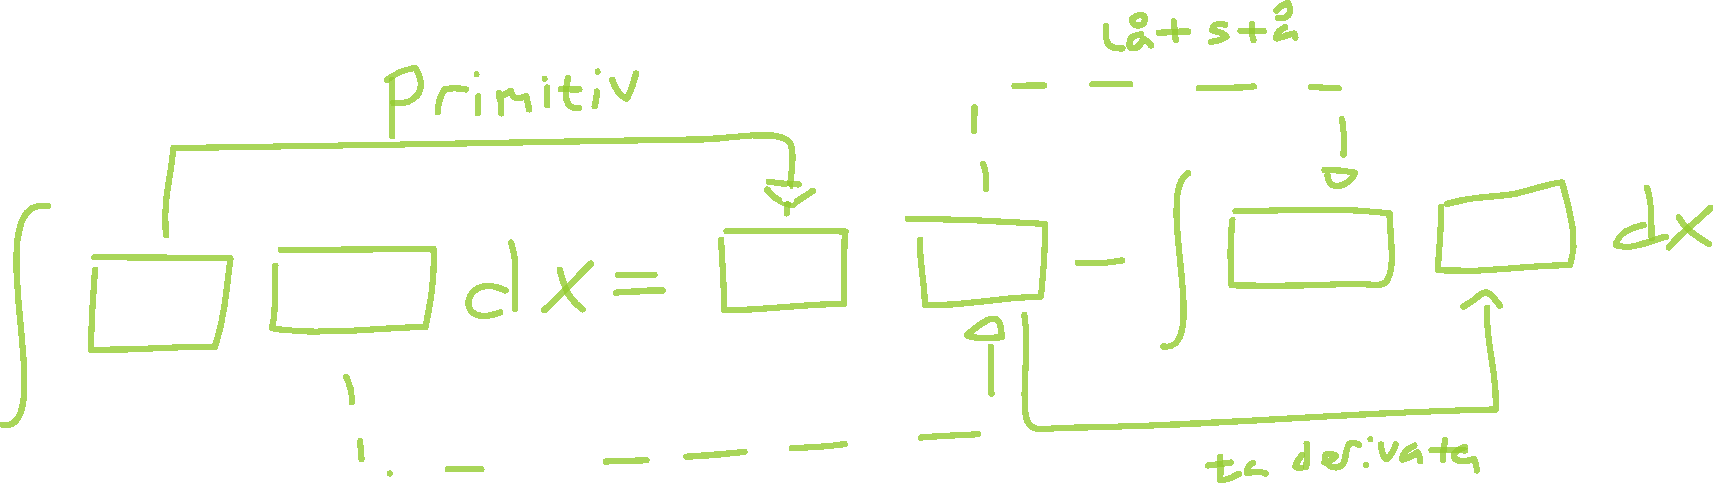
\includegraphics[scale=0.5]{img/img1.pdf}

\subsection{Exempel (Skjut in en etta)}
$$ \int{\ln \abs{x} dx}=\int{1\times \ln{\abs{x}} dx} = x \times \ln{\abs x} - \int{x \times \f 1x dx} = x \ln{\abs{x}} - x + C $$

\subsection{Exempel (Upprepad partiell integration)}
$$ \int{x^3 e^{-2x} dx} = \int{e^{-2x}x^3 dx} = \f{e^{-2x}}{-2} \times x^3 - \int{\f{e^{-2x}}{-2} 3x^2 dx} = \f{e^{-2x}}{-2}\times x^3 - \left( \f{e^{-2x}}{(-2)^2}\times 3x^2 - \int{\f{e^{-2x}}{(-2)^2} 6x dx}\right)=$$
$$ = \f{e^{-2x}}{-2}x^3  - \f{e^{-2x}}{(-2)^2} 3x^2 + \f{e^{-2x}}{(-2)^3}6x - \int{\f{e^{-2x}}{(-2)^3} 6 dx}=$$
$$ = \f{e^{-2x}}{-2}x^3  - \f{e^{-2x}}{(-2)^2} 3x^2 + \f{e^{-2x}}{(-2)^3}6x - \f{e^{-2x}}{(-2)^4}\times 6 + C=$$
$$ -e^{-2x}\left(\f{x^3}2 + \f{3x^2}4 + \f{3x}4 + \f 38 + C\right) $$
\\
Eller ta allt i ett steg, om man så vill:\\
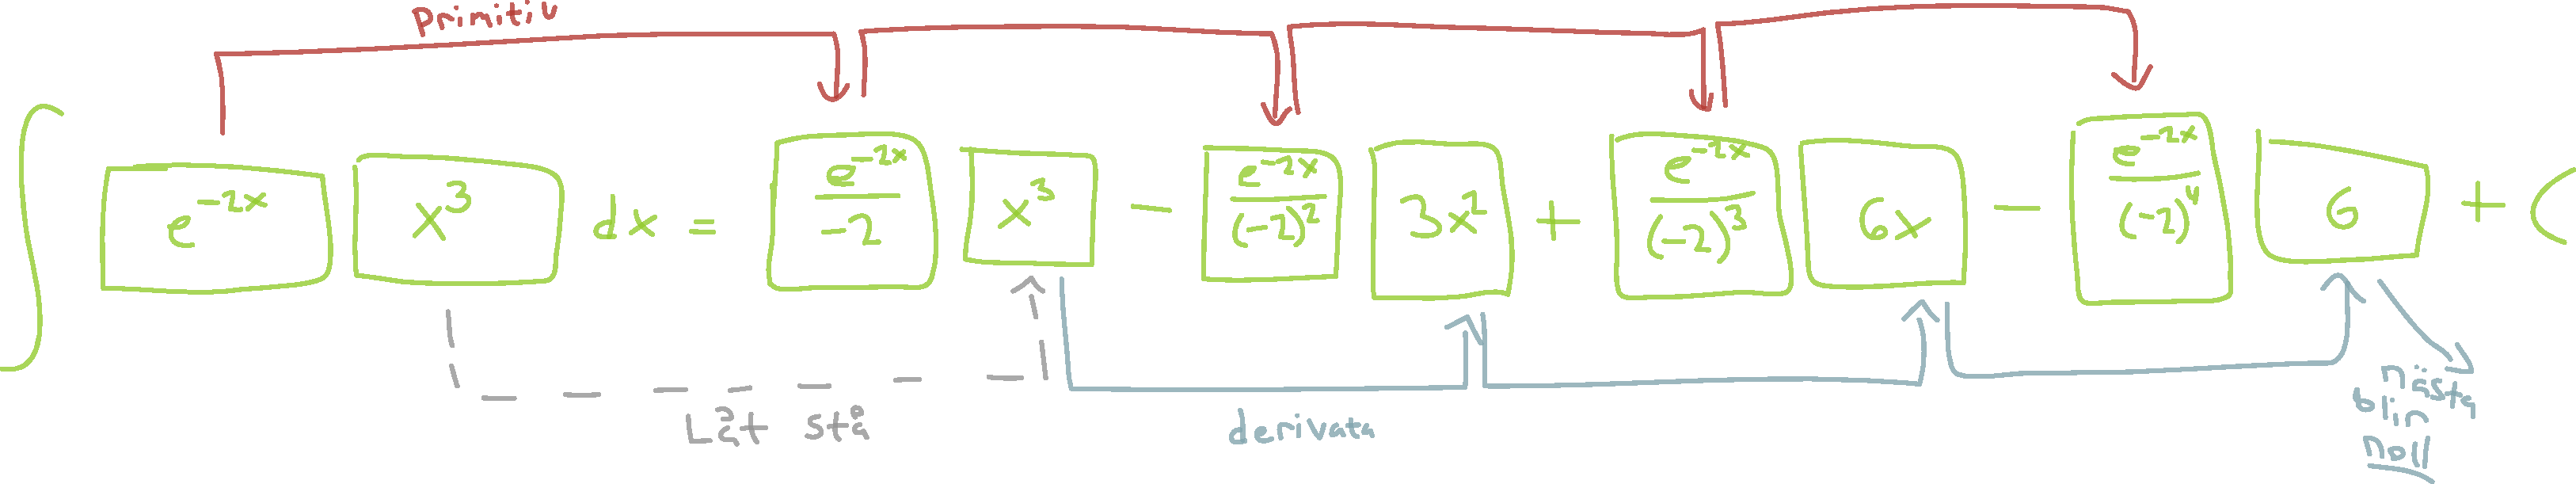
\includegraphics[scale=0.3]{img/img2.pdf}

\section{Variabelbyte (= kedjeregeln baklänges)}
Uträkningen $\int{\cos(x^3+1)3x^2 dx} = \sin\left(x^3+1\right) + C$ innefattar två steg:
\begin{itemize}
    \item Känna igen att $3x^2$ är derivatan av $x^3+1$
    \item Beräkna primitiv till cosinusfunktionen (dvs $\int{\cos t dt} = \sin t + C$)
\end{itemize}

\subsection{Praktiskt skrivsätt}
$$ \int{\cos(x^3+1)3x^2 dx} = \bmat{t=x^3+1 \\ \f{dt}{dx} = 3x^2 \\ dt=3x^2 dx} = \int{\cos t dt} = \sin t + C = \sin (x^3+1) + C$$

\subsection{Exempel}
$$ \int{dx \over 1+e^x} = \bmat{x=\ln t\ (t>0)\\ \f{dx}{dt} = \f 1t \\ dx = \f{dt}t} = \int{dt \over (1+t)t} = \int{\f{(1+t)-t}{(1+t)t}dt}  =$$
$$=\int{\pa{\f 1t - \f 1{1+t}}dt} = \ln \abs t - \ln \abs{1+t} + C = \ln t - \ln (1+t) + C = x - \ln {1+e^x}$$

\subsection{Exempel}
$$ \int{\f{x}{x^2 + 6x + 13}dx} = \int{\f{x}{(x+3)^2+4}dx} = \bmat{ t=x+3 \\ \f{dt}{dx} = 1 \\  dt=dx} =\int{\f{t-3}{t^2+4}dt} = \int{\f t{t^2+4}dt} - 3\int{\f 1{t^2+4}dt}$$
$$A = \int{\f t{t^2+4}dt}$$
$$B = 3\int{\f 1{t^2+4}dt}$$
$$ A=\bmat{u=t^2+4 \\ \f{du}{dt} = 2t \\ du=2t\ dt} = \int{\f 12 du \over u} = \f 12 \ln \abs u + C = \f 12 \ln\pa{t^2+4}+C_1 = \f 12 \ln\pa{(x+3)^2+4} + C_1 =$$
$$ B=\int{\f 1{4(\f{t^2}4 + 1)dt }= \f 14 \int{\f 1{\pa{\f t2}^2 + 1} dt}} = \bmat{v=\f t2 \\ \f{dv}{dt} \\ dt=2v} = \f 14 \int{\f 1 {v^2+1} 2v} = $$
$$=\f 12 \arctan v + C_2 = \f 12 \arctan \f t2 + C_2 = \f 12 \arctan \f{x+3}2 + C_2 $$
\end{document}
